\begin{figure}
    \centering
    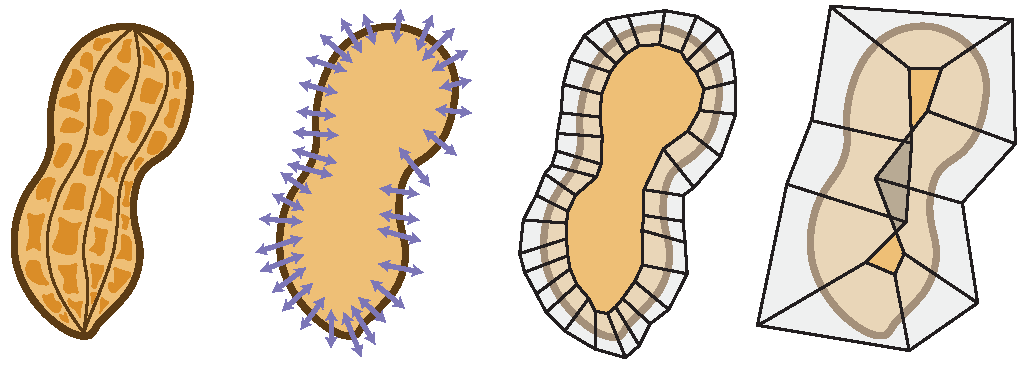
\includegraphics[width=\linewidth]{prism-tex/figs/pipeline}
    \caption{Overview of our algorithm. We start from a triangle mesh, find directions of extrusion, build the shell, and optimize to simplify it.}
    \label{prism:fig:pipeline}
    
\end{figure}

\section{Method}\label{prism:sec:method}
Our algorithm (Figure~\ref{prism:fig:pipeline}) converts a self-intersection free, orientable, manifold triangle mesh $\T = \{V_\T,F_\T\}$, where $V_\T$ are the vertex coordinates and
$F_\T$ the connectivity of the mesh, into a shell composed of generalized prisms $\S = \{(B_\S,M_\S,T_\S),F_\S\}$, where $B_\S$, $M_\S$, $T_\S$ are bottom, middle, and top surfaces of the shell, 
consisting of bottom, middle, and top  triangles of the prisms,
and $F_\S$  is the connectivity of the prisms (Figure \ref{prism:fig:corona}).
The algorithm initially generates a shell $\S$ whose middle surface $M_\S$ has the same geometry as the input surface $\T$ (possibly with refined connectivity),
and then optimizes it while ensuring that $\T$ is contained inside and projects bijectively to $M_\S$. The shell induces a volumetric vector field $\V$ and a projection operator $\P$ in the interior of each of its prisms (Section \ref{prism:sec:projection}). This output can be used directly in many geometry processing tasks, as we discuss in detail in Section~\ref{prism:sec:applications}.

\begin{figure}
    \centering
    \includegraphics[width=0.9\linewidth]{prism-tex/figs/corona}
    \caption{Example of the top (left, outer) and bottom (right, inner) surface of the prismatic shell.}
    
    \label{prism:fig:corona}
\end{figure}


We first introduce the definition of our projection operator $\P$ and the conditions required for bijectivity of its restrictions to sections of the shell (Section \ref{prism:sec:projection}). We then define shell validity (Section \ref{prism:sec:strong}), present our algorithm for creating an initial shell (Section\ \ref{prism:sec:initialization}) and optimizing it to decrease the number of prisms (Section \ref{prism:sec:optimization}).
To simplify the exposition,
we initially assume that our input triangle mesh does not contain \emph{singular points} (defined in Section~\ref{prism:sec:initialization}) and boundary vertices, and we explain how to modify the algorithm to account for these cases in sections \ref{prism:sec:singularities} and \ref{prism:sec:boundaries}.

\subsection{Shell and Projection}
\label{prism:sec:projection}

Let us consider a single generalized prism $\Prism$ in a prismatic layer $\S$ (Figure \ref{prism:fig:prism_decomposition} left). The generalized prism $\Prism$ is defined by the position of the vertices of three triangles, one at the top, with coordinates $t_1,t_2,t_3$, one at the bottom, with coordinates $b_1,b_2,b_3$, and one in the middle, implicitly defined by a per-vertex parameter $\alpha_i \in [0, 1]$, with coordinates $m_i = \alpha_i t_i + (1-\alpha_i) b_i, i=1,2,3$. We will call the top (bottom) ``half'' of the prism \emph{top (bottom) slab} (we refer to Appendix~\ref{app:dblayer} for an explanation on why we need two slabs).
For brevity, we will refer to a generalized prism as a prism.

% Without loss of generality, we will describe our algorithm only for the top half of the prism $\Prism$ denoted $\H$ since the other half of the construction is symmetric.

\begin{figure}
    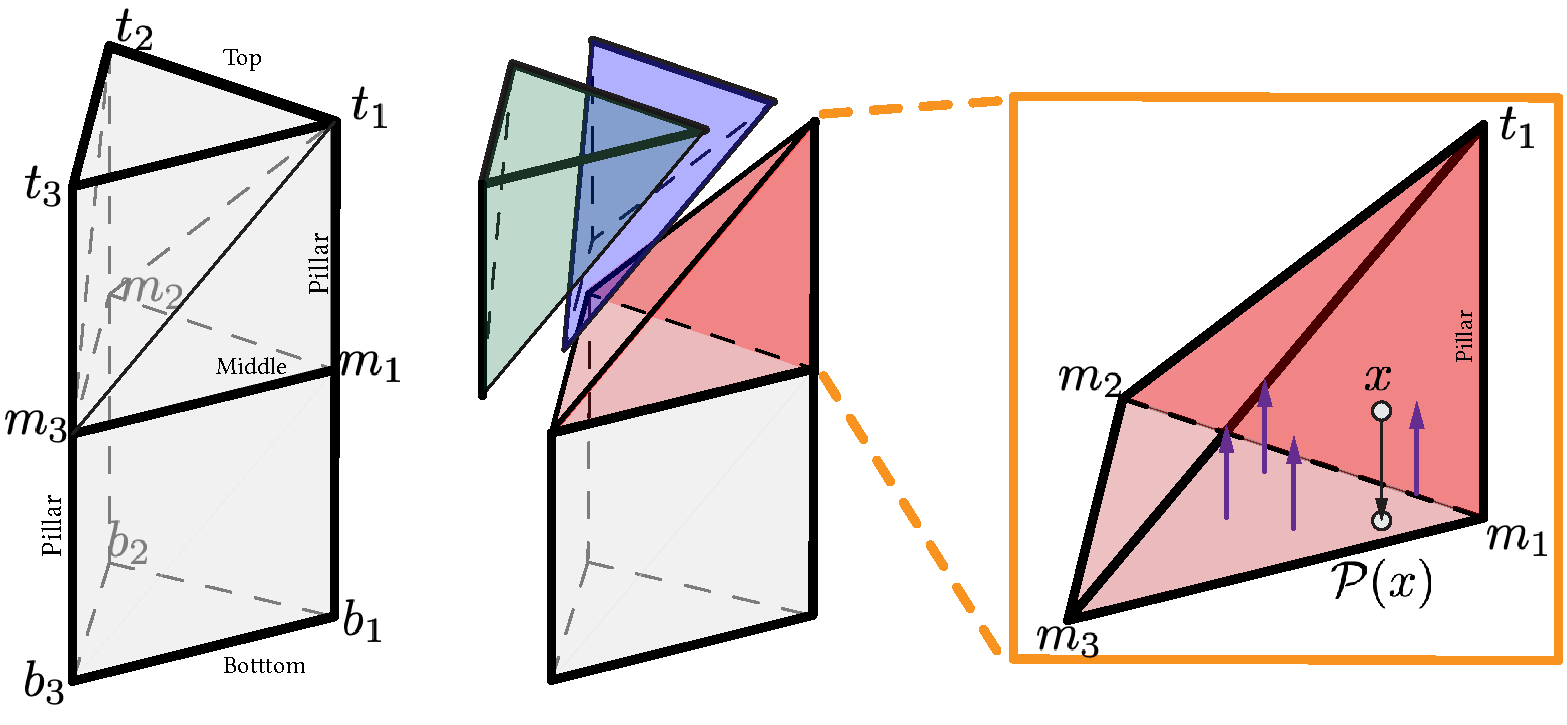
\includegraphics[width=\linewidth]{prism-tex/figs/prism_projection}
    \caption{A prism $\Prism$ (left) is decomposed into 6 tetrahedra (middle, for clarity, we only draw the 3 tetrahedra of the top slab). Each tetrahedron has a constant vector field in its interior (pointing toward the top surface), which is parallel to the only pillar of the prism that contains the point.}
    \label{prism:fig:prism_decomposition}
    
\end{figure}

 \paragraph{Decomposition in Tetrahedra} We decompose each prism $\Prism$ into 6 tetrahedra (3 in the top slab and 3 in the bottom one, Figure~\ref{prism:fig:prism_decomposition} middle), using one of the patterns in \cite[Figure 4]{dompierre1999subdivide}. The patterns are identified by the orientation (rising/falling) of the two edges cutting the side faces of the prism. While, for a single prism, any decomposition would be sufficient for our purposes, we need a consistent tetrahedralization between neighboring prisms to avoid inconsistencies in the projection operator. To resolve this ambiguity, we use the technique proposed in \cite{garimella2000boundary}: we define a total ordering over the vertices of the middle surface of $\Prism$ (naturally, we use the vertex id) and split (for each half of the prism) the face connecting vertices $v_1$ and $v_2$ with a rising edge if $v_1 < v_2$ and a falling edge otherwise. 

\paragraph{Forward and Inverse Projection}
% \ZJ{multi-value definition comment.
% Vector Field is defined piecewise, but the projection is unique.}
We define a piecewise constant vector field $\V$ inside the decomposed prism,
by assigning to each tetrahedron $\Tet_j^{\Prism}$, $j=1,\hdots,6$,
the constant vector field defined by the only edge of $\Tet_j^{\Prism}$ which is a \emph{oriented pillar} of $\Prism$ connecting the bottom surface to the top surface passing through the middle surface). That is, for any $p\in \Tet_j^{\Prism}$
\begin{equation}
    \label{eq:V}
    \V(p) = t_i - b_i,
\end{equation}
where $i$ is the index of the vertex corresponding to the pillar edge of $\Tet_j^{\Prism}$.
Note that {$\V$ is constant on each tetrahedron and might be discontinuous on the boundary: we formally define the value of $\V$ on the boundary as any of the values of the incident tetrahedra. This choice does not affect our construction.}
{T}here is exactly one {integral (poly-)line} passing through each point of the prism if
all the decomposed tetrahedra have positive volumes
(Theorem~\ref{thm:projection}). This allows us to define
the \emph{projection operator} $\P(p)$ for a point $p \in \Prism$ as the intersection of the {integral line} $f_p(t)$ of the vector field $\V$ passing through $p$, with the middle surface of $\Prism$ (Figure~\ref{prism:fig:advection}). 
%
\begin{figure}
    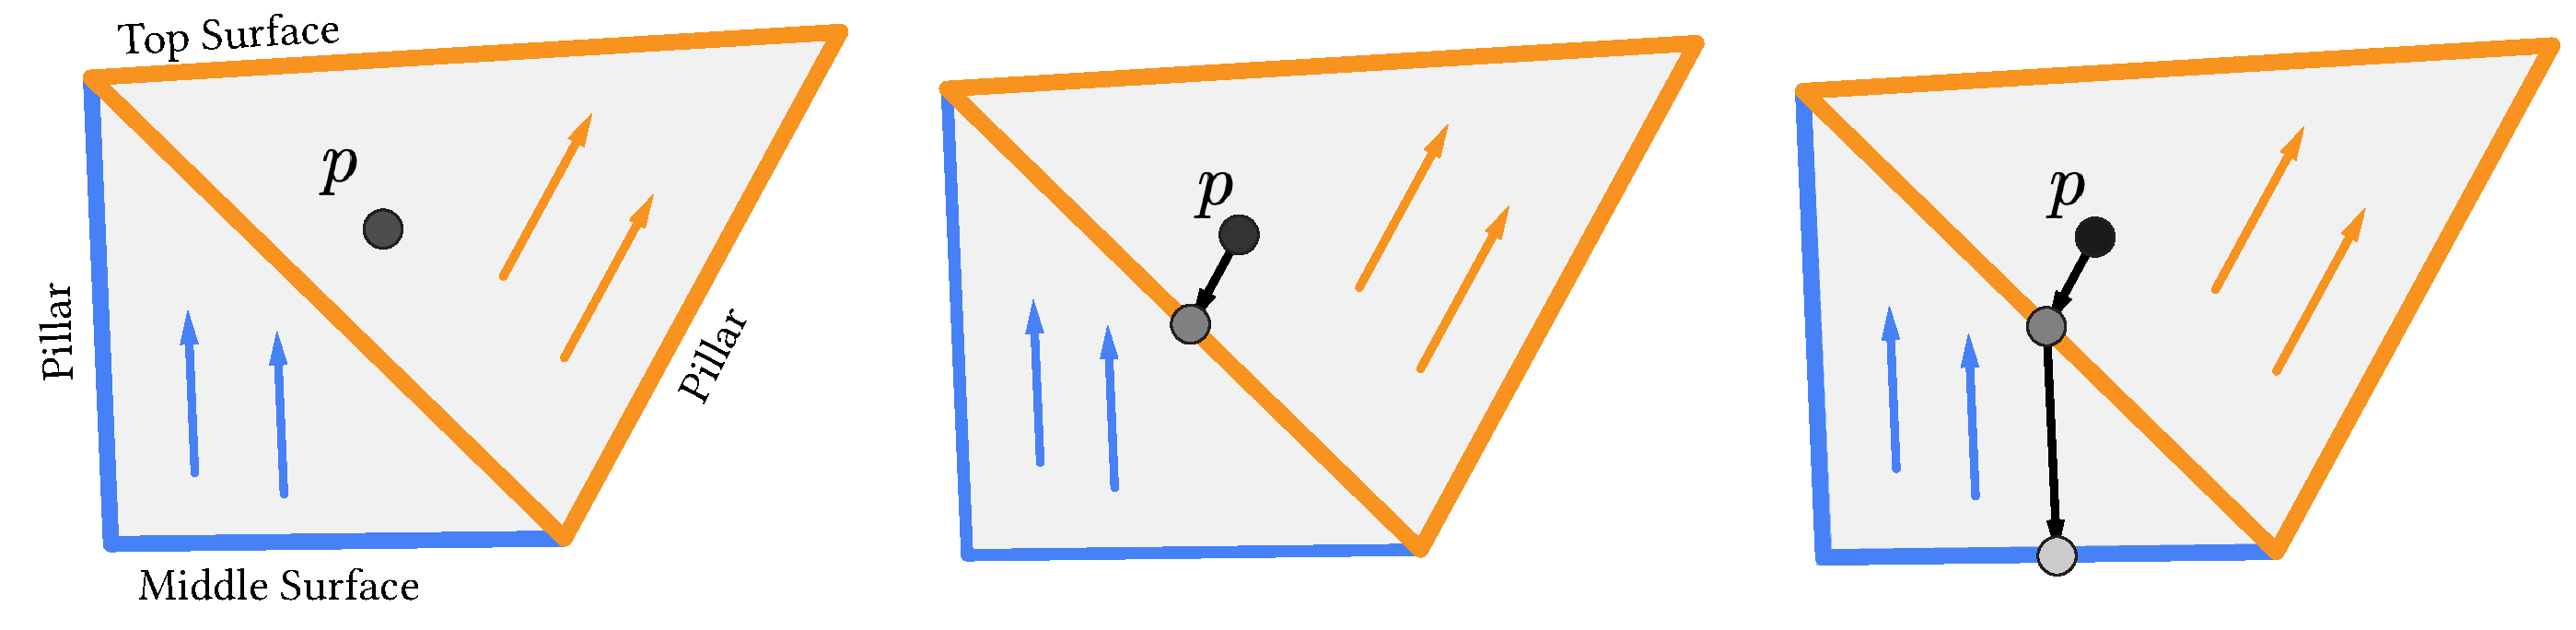
\includegraphics[width=\linewidth]{prism-tex/figs/projection}
    \caption{A point $p$ (left) is traced through $\V$ inside the top part of the shell. A ray with $p$ as origin and $\V$ as direction is cast inside the orange tetrahedron (middle). The procedure is repeated (on the blue tetrahedron) until the ray hits a point in the middle surface (right).}
    \label{prism:fig:advection}
    
\end{figure}
%
% \begin{wrapfigure}{r}{width=0.3\linewidth}
%     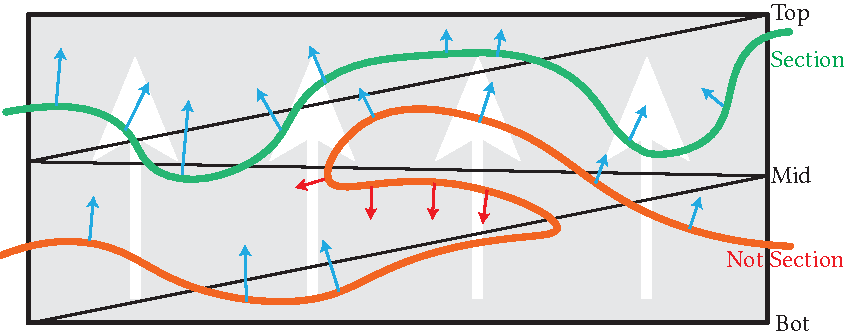
\includegraphics[width=\linewidth]{prism-tex/figs/not-section-illustrate}
% \caption{Example of being a section (green) and not a section (red).}
% \end{wrapfigure}
%
Intuitively, we can project any mesh that does not fold in each prism (Figure~\ref{prism:fig:not_section}) to the middle surface.
\begin{figure}
    \centering
    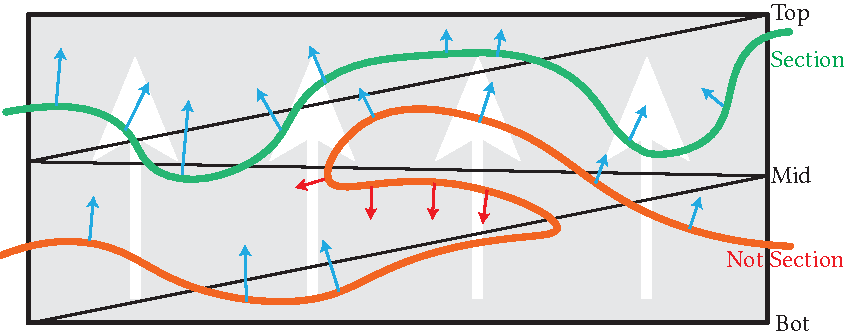
\includegraphics[width=0.8\linewidth,draft=false]{prism-tex/figs/not-section-illustrate}
    \caption{A 2D illustration for the normal dot product condition. The blue arrows agrees with the background vector field (white arrows), while the red arrows do not agree.}
    \label{prism:fig:not_section}
    
\end{figure}
Formally, we introduce the following definition, to describe this property in terms of the triangle normals of the mesh.

With a slight abuse of the notation, for meshes and collections of prisms $A$ and $B$, we use $A \cap B $ to denote the intersection of their corresponding geometry.

\begin{definition}
\label{def:section}
A \emph{section} $\hat{\T}$ of a prism $\Prism$ is a manifold triangle mesh whose intersection with $\Prism$ is a simply connected submesh $\hat{\T} \cap \Prism$ whose single boundary loop is contained in the boundary of $\Prism$, excluding its top and bottom surface, and such that for every point $p \in \hat{\T} \cap \Prism$ the dot product
between the face normal $n(p)$ and the vector field $\V(p)$ is strictly positive. Similarly, a triangle mesh $\hat{\T}$ is a \emph{section of a shell $\S$}, if it is a section of all the prisms of $\S$.
\end{definition}
Note that this definition implies that all sections are contained inside the shell.
% that is, the union of all prisms minus the intersection region of non-adjacent prisms (light gray area in Figure~\ref{prism:fig:pipeline)}\ZJ{Move this sentence}.
{Additionally, the definition implies that the section does not intersect with either bottom or top surface. 
However, our definition allows for the bottom or top surface to self-intersect. 
The intersection of the shell does not invalidate the \emph{local} definition of projection since it is defined per prism.
Allowing intersections is crucial to an efficient implementation of our algorithm since it allows us to take advantage of a static spatial data structure in later stages of the algorithm (Section~\ref{prism:sec:optimization}).
}

 

\begin{theorem}
If all  6 tetrahedra $\Tet_j^{\Prism}$ in a decomposition of a prism $\Prism$ have positive volume,
then the projection operator $\P$ defines a bijection between any section $\hat{\T}$ of $\Prism$ and the middle triangle of the prism ($M$ in Figure~\ref{prism:fig:projection_sections}).
\label{thm:projection}
\end{theorem}
\begin{proof}
    \label{app:projection}
    Consider the unique (up to symmetry) piece-wise affine map $T$ deforming $\Prism$ into a reference prism $\hat\Prism = \{u,v \geq 0|u+v \leq 1\} \times [-1,1]$, identifying the bottom surface of $\hat\Prism$ as $z=-1$, middle surface as $z=0$, and top surface as $z=1$.
    Let $T_{\Tet}$ be the affine map mapping tetrahedron $\Tet$ to the reference prism.
    Since the volume of all $\Tet$ is positive by assumption, the map $T$ is bijective and orientation preserving. 
    In particular, $T$ transforms $\V(p)$ to the const vector $e_z = (0,0,1)$ since the edges of the prism are mapped to axis aligned edges of the reference prism. The projection operator $\P(p)$ can thus be equivalently defined as $\P(p) = T^{-1}(\P_z(T(p)))$, where $\P_z$ is the projection over the $z$-axis in the reference prism. 
    $\P_z$ is bijective if the piecewise linear mesh intersecting $\Prism$ is composed of triangles with positive area (and the boundaries are mapped to the boundaries) \cite{lipman2014bijective}, after being mapped to the reference $\Prism$ and projected by $\P_z$. In the reference domain, having positive area after projection (with a fixed boundary) is equivalent to that the dot product between the projection direction and the normal of every face is positive. In the top half of $\Prism$, $\P_z$ is bijective if for every point $T(p), p \in f$ $T(n_p)\cdot [0,0,1] = T(n_p) \cdot T(\V(p)) > 0$  which holds since $ n_p \cdot \V(p) > 0$ (from the definition of section) and the fact that $T$ is orientation preserving and thus not changing the sign of the dot product.
\end{proof}

The \emph{inverse projection operator} $\P^{-1}$ is defined for a section $\hat{\T}$ as the inverse of the forward projection
restricted to $\hat{\T}$. %, $\P: \hat{\T} \rightarrow \T$ is bijective.
It can be similarly computed by tracing the vector field in the opposite direction, starting from a point in the middle surface of the prism. Note that, differently from the inverse Phong projection \cite{panozzo2013weighted, kobbelt1998interactive}, whose solution depends on the root-finding of a quadric surface, our shell has an explicit form for the inverse and does not require a numerical solve. The combination of forward and inverse projection operators allows to bijectively map between any pair of sections, independently of their connectivity (Figure \ref{prism:fig:projection_sections}). An interesting property of our forward and inverse projection algorithm, which might be useful for applications requiring a provably bijective map, is that our projection could be evaluated exactly using rational arithmetic.

%%%%%%%%%%

\begin{figure}
    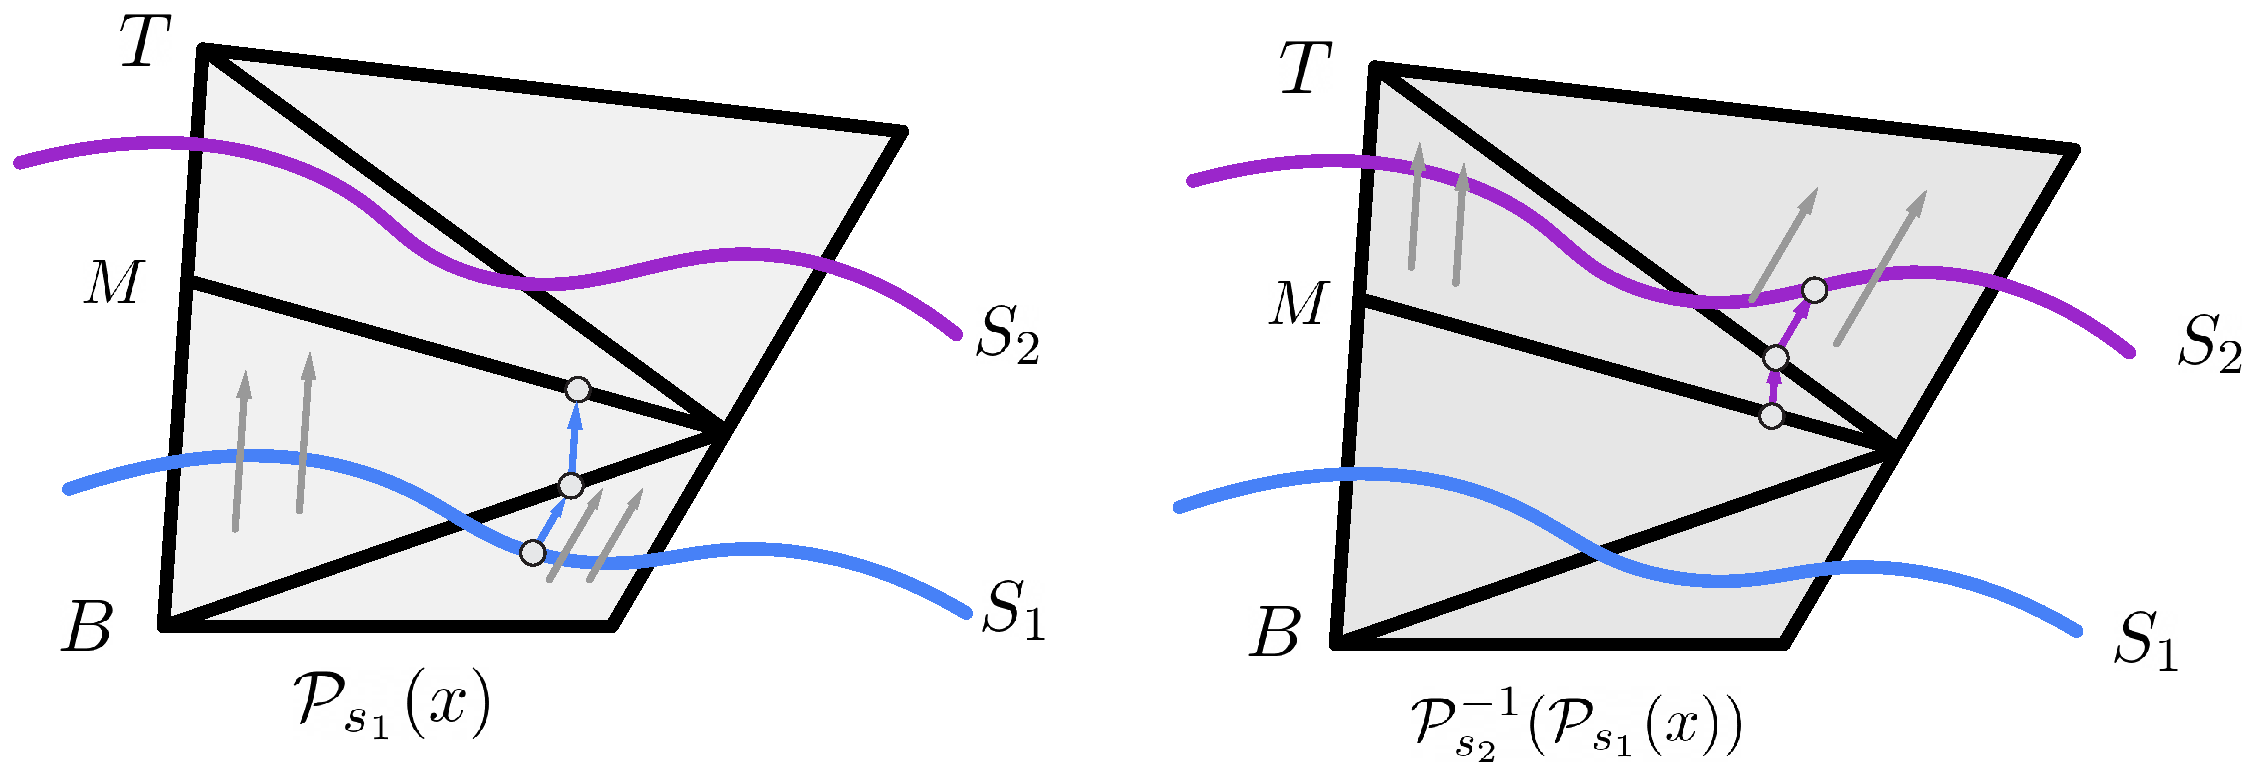
\includegraphics[width=\linewidth]{prism-tex/figs/composition}
    \caption{The composition $\P^{-1}_{\S_2}(\P_{\S_1}(x))$ with $x \in \S_1$, of a direct and an inverse projection operator defines a bijection between two sections $\S_1$ and $\S_2$.}
    \label{prism:fig:projection_sections}
    
\end{figure}

{
\subsection{Validity Condition}
\label{prism:sec:strong}

Shell, projection operator, section definitions, and the bijectivity condition (Theorem~\ref{thm:projection}) are dependent on a specific tetrahedral decomposition, which depends on vertex numbering.

To ensure that our shell construction is independent from the vertex and face order, we define the validity of a shell by accounting for all 6 possible tetrahedral decompositions \cite[Figure 4]{dompierre1999subdivide}}.

\begin{definition}\label{def:validshell}
% \paragraph{Validity}
We say that a prismatic shell $\S$ is \emph{valid with respect to a mesh $\hat\T$} if it satisfies two conditions for each prism.
\begin{enumerate}
    \item[I1] \emph{Positivity}. The volumes of  24 tetrahedra (Appendix \ref{app:I1}) corresponding to  6 tetrahedral decompositions are positive.
    \item[I2] \emph{Section.} $\hat\T$ is a section of $\S$ for all 6 decompositions.
\end{enumerate}
\end{definition}
If a shell is valid, from I1, I2, then by Theorem \ref{thm:projection}, it follows that any map between sections induced by the projection operator $\P$ is bijective.

I2 ensures that the input mesh is a \emph{valid section} independently from the decomposition, that is, we require the dot product to be positive with respect to all \emph{three} pillars of a prism inside the convex hull. An interesting and useful side effect of this validity condition is that it ensures the bijectivity of a natural nonlinear parametrization of the prism interior (Appendix \ref{app:bilinear}, Figure~\ref{prism:fig:displacement-mapping}).

\subsection{Shell Initialization}
\label{prism:sec:initialization}

We now introduce an algorithm to compute a \emph{valid} prismatic shell $\S = \{(B_\S,M_\S,T_\S),F_\S\}$ with respect to a given triangle mesh $\T = \{V_\T,F_\T\}$ such that $\T$ is geometrically identical to the middle surface of $\S$.  We assume that the faces of the triangle mesh are consistently oriented.

\paragraph{Extrusion Direction.} The first step of the algorithm is the computation of an extrusion direction for every vertex of $\T$. These directions are optimized to be pointing towards the \emph{outside} of the triangle mesh (which we assume to be orientable), that is,
they must have a positive dot product with the normals of all incident faces. More precisely, for a vertex $v$, we are looking for a direction $d_v$ such that $d_v \cdot n_f > 0$ for each adjacent face $f$ with normal $n_f$. We can formulate this as the optimization problem
\begin{equation}
\label{eq:OPT}
\begin{split}
    \max_{d_v}& \min_{f \in N_v} n_f \cdot d_v,\\
    \text{s.t. }&\quad n_f \cdot d_v \geq {\epsilon}, \qquad \forall f \in N_v\\
               &\quad  \|d_v\|^2 = 1.
\end{split}
\end{equation}

With slack variable $t$, Problem \ref{eq:OPT} can be rewritten as

$$\max_t t;\; d_v n_f \geq t, \|d_v\| = 1, t \geq {\epsilon}.$$

In the admissible region, substituting 
$t = 1/s$, 
$$\min_s s;\; s d_v n_f \geq 1, \|d_v\| = 1, {0< s \leq 1/\epsilon}.$$
Substituting $x=s d_v$ (thus $\|x\| = s\|d\| = s$), we obtain the QP problem \ref{eq:QP}. Note that the lower bound on $s$ is implied from $s d_v n_f \geq 1$, and the upper bound $\|x\| < 1/\epsilon$ is checked a posteriori.

A solution, if it exists, can be found solving the following quadratic programming problem
\begin{equation}
\label{eq:QP}
\begin{split}
    \min&\quad \|x\|^2,  \\
    \text{s.t.}&\quad \mathbf{C} x \geq 1,
\end{split}
\end{equation}
with $d_v = x / \|x\|$ and $\mathbf{C}$ the matrix whose rows are the normals $n_f$ of the faces in the 1-ring $N_v$ of vertex $v$. Solutions not satisfying $\|x\| \leq 1/\epsilon$ needs to be discarded. The QP can be solved with an off-the-shelf solver\cite{osqp,cheshmi2020nasoq}, and in particular it can be solved exactly \cite{gartner2000efficient} to avoid numerical problems. Note that the Problem \eqref{eq:OPT} is studied in a similar formulation in~\cite{aubry2008most} but their solution requires tolerances in multiple stages of the algorithm to handle cospherical point configurations.




The admissible set of \eqref{eq:OPT} might be empty for a vertex $v$,
that is, no vector $d_v$ satisfies $\mathbf{C}d_v\geq\epsilon$. 
In this case we call $v$ a \emph{singularity}. For example, Figure \ref{prism:fig:singularity_example} shows a triangle mesh containing a singularity: there exist no direction whose dot product with the adjacent face normals is positive. To simplify the explanation, we assume for the remainder of this section that $\T$ does not contain singularities and also that it does not contain boundaries: we postpone their handling to sections \ref{prism:sec:singularities} and \ref{prism:sec:boundaries}.

\begin{proposition}\label{thm:I1}
Let $\T$ be a closed (without boundary) triangle mesh without singularities and $\N$ be a per-vertex displacement field satisfying $\mathbf{C} \N_i > 0$ for every vertex $v_i$ of $\T$. 
Then there exist a strictly positive per-vertex \emph{thickness} $\delta_i$ such that vertices $t_i$ and $b_i$ obtained by displacing $v_i$ by $\delta_i$ in the direction of $\N_i$ and in the opposite direction, define a shell that satisfies invariant I1.
\end{proposition}
\begin{proof}
    \label{app:I1}
    For simplicity, we will show that a uniform lower bound $\delta$ for all vertices exists. By consider a triangle of $T$, extruded over the displacement field $\N$, we obtain a generalized half prism with six vertices
    $0$, $e_1$, $e_2$, $\delta n_0$, $e_1$ + $\delta n_1$, $e_2 + \delta$ $n_2$, with $\delta$ a positive constant. The indices of the tetrahedra are:
    (0 ,2, 3, 4), 
    (0 ,3, 4, 5), 
    (0 ,1, 5, 3), 
    (0 ,1, 2, 3), 
    (1 ,2, 3, 4), 
    (0 ,1, 2, 4), 
    (0 ,1, 5, 4), 
    (1 ,3, 4, 5), 
    (1 ,2, 3, 5), 
    (0 ,2, 5, 4), 
    (0 ,1, 2, 5), 
    (2 ,3, 4, 5). 
    
    For a sufficiently small $\delta$, the linear term will dominate the higher power of $\delta$, which we omit. 
    The dominant volume terms are listed in the following table: ($e_{ij} := e_j - e_i$)
    
    \vspace{1em}
    {
    % \begin{table}[t]
    \footnotesize
        \centering
        {
    \begin{tabular}{|l|l|l|}
    \hline
    (0 ,2, 3, 4)&\text{vol1}$( 0,e_2,\delta  n_0,e_1 + \delta  n_1)           $&$ \delta \langle e_2,n_0,e_1\rangle$\\             
    (0 ,3, 4, 5)&\text{vol2}$( 0,\delta  n_0,e_1 + \delta  n_1,e_2 + \delta n_2)   $&$ \delta \langle n_0,e_1,e_2\rangle $\\
    (0 ,1, 5, 3)&\text{vol3}$( 0,e_1,e_2 + \delta n_2,\delta  n_0)            $&$ \delta \,\langle e_1,e_2,n_0\rangle  $\\
    (0 ,1, 2, 3)&\text{vol4}$( 0,e_1,e_2,\delta  n_0)                    $&$ \delta \langle e_1,e_2,n_0\rangle                           $\\
    (1 ,2, 3, 4)&\text{vol5}$( e_1,e_2,\delta  n_0,e_1 + \delta  n_1)         $&$ \langle e_{12}, \delta  n_0 - e_1, \delta n_1\rangle            $\\ 
    && $=\delta \langle e_2, -e_1, n_1\rangle     $\\
    (0 ,1, 2, 4)&\text{vol6}$( 0,e_1,e_2,e_1 + \delta  n_1)             $&$ \delta \langle e_1,e_2,n_1\rangle                             $\\
    (0 ,1, 5, 4)&\text{vol7}$( 0,e_1,e_2 + \delta n_2,e_1 + \delta  n_1)     $&$ \langle e_1,e_2 + \delta n_2, \delta  n_1\rangle                  $\\ 
    &&$ =\delta \langle e_1,e_2,n_1\rangle                                           $\\
    (1 ,3, 4, 5)&\text{vol8}$( e_1,\delta  n_0,e_1 + \delta  n_1,e_2 + \delta n_2) $&$ \delta \langle \delta  n_0 -e_1, n_1, e_{12} + \delta n_2\rangle    $\\ 
    &&$ = \delta \langle -e_1, n_1, e_2\rangle                                   $\\
    (1 ,2, 3, 5)&\text{vol9}$( e_1,e_2,\delta  n_0,e_2 + \delta n_2)          $&$ \langle e_{12}, \delta  n_0 - e_1, e_{12} + \delta n_2 \rangle $\\
    &&$ =\delta \langle e_{12}, \delta  n_0 - e_1, n_2\rangle $\\
    &&$ =\delta \langle e_2, - e_1, n_2\rangle $\\
    (0 ,2, 5, 4)&\text{vol10}$( 0,e_2,e_2 + \delta n_2,e_1 + \delta  n_1)     $&$ \delta \langle e_2, n_2, e_1\rangle$ \\
    (0 ,1, 2, 5)& \text{vol11}$( 0,e_1,e_2,e_2 + \delta n_2)$
                                                      &$ \delta \langle e_1,e_2,n_2\rangle $\\
    (2, 3, 4, 5)&\text{vol12}$( e_2,\delta  n_0,e_1 + \delta  n_1,e_2 + \delta n_2) $&$ \langle \delta  n_0 - e_2, \delta  n_1-e_{12}, \delta  n_2\rangle      $\\
    &&$ =\delta \langle - e_2, e_1, n_2\rangle$
                                                      \\
                                                      \hline
    \end{tabular}}
    % \end{table}
    \vspace{1em}
    }
    
    
    For all the 12 tetrahedra the linear term is multiplied by a determinant containing the edges of the prism. We check directly that all these determinants are positive due to the assumption that $\mathbf{C} \N_i > 0$.
    
\end{proof}




\paragraph{Initial Thickness}
We first show that a strictly positive per-vertex thickness $\delta$ exists for a shell $\S$ with $\T$ as its middle surface, and then discuss a practical algorithm to realize it.

\begin{theorem}
\label{thm:thickness}
Given a closed, orientable, self-intersection free triangle mesh $\T$ such that for all its vertices  Problem \eqref{eq:OPT} has a solution, a shell $\S$ exists such that $\T$ is the middle surface and there exist a strictly positive per-vertex thickness $\delta$.
\end{theorem}
\begin{proof}

    Consider a ball around a point $p$ of the middle face $M$ of the prism.  
    If the radius $r(p) > 0$ is sufficiently small, it contains, at most, a single vertex of $M$, and parts of incident  faces. As $M$ is compact, there is a minimal value of $r$ on $M$, and it is positive. 
    The line along the normal, passing through $v$, intersects incident faces at $v$ so it cannot intersect them at any other point. Thus, the top and bottom prism vertices can be obtained by displacing $V$ by $r$ in either direction along the normal. 
    Consider the $r$-neighborhood of the $M$, i.e. the union of all balls of radius $r$ centered at 
    points of $M$. This is a convex set, containing only $M$ and parts of vertex-adjacent faces. 
    All top and bottom prism vertices are in this set. Thus tetrahedra connecting these vertices are also in the set, i.e., complete prisms. The fact that tetrahedra are nondegenerate is established in Proposition~\ref{thm:I1}.
    \end{proof}


To find a valid per-vertex thickness $\delta_i$ to construct the top surface, we initially cast a ray in the direction of $\N$ for each vertex and measure the distance to the first collision with $\T$ (and cap it to a user-defined parameter $\delta_{max}$ if no collision is found).
An initial top mesh is built with this extrusion thickness; then we test whether any triangle in the top surface intersects $\T$, through triangle-triangle overlap test \cite{guigue2003fast},
and iteratively shrink $\delta_i$ in this triangle by 20\% until we find a thickness that prevents intersections between the input and the top surface. Analogously, we build the bottom shell along the opposite direction. {Note that the thickness of a vertex for the top and bottom surface can be different.}

\paragraph{Validity of the Initial Shell}
Proposition~\ref{thm:I1} and Theorem~\ref{thm:thickness} ensure that the initial shell constructed using a displacement field $\N$ obtained by solving \eqref{eq:QP}, satisfies property I1. However, $\T$ might not formally satisfy the conditions for being a section of $\S$, despite being identical to the middle surface of $\S$, due to our definition of the projection operator $\P$.
%
The reason for this can be seen in Figure \ref{prism:fig:closed}.
After the initialization, the middle surface is the input mesh. Thus every prism $\Prism$ corresponds to a triangle $T_\Prism$ of $\T$. The intersection $\Prism \cap \T$, required to check if $\T$ is a section of $\Prism$ (Definition \ref{def:section}) contains points from both $T_\Prism$ and its 1-ring neighborhood.

The projection operator (and thus the definition of the section) is based on all tetrahedral decompositions of $\Prism${;} it is possible that multiple tetrahedra (with different vector field values in $\V$) overlap on the boundary of $\Prism$. 


\begin{figure}\centering
    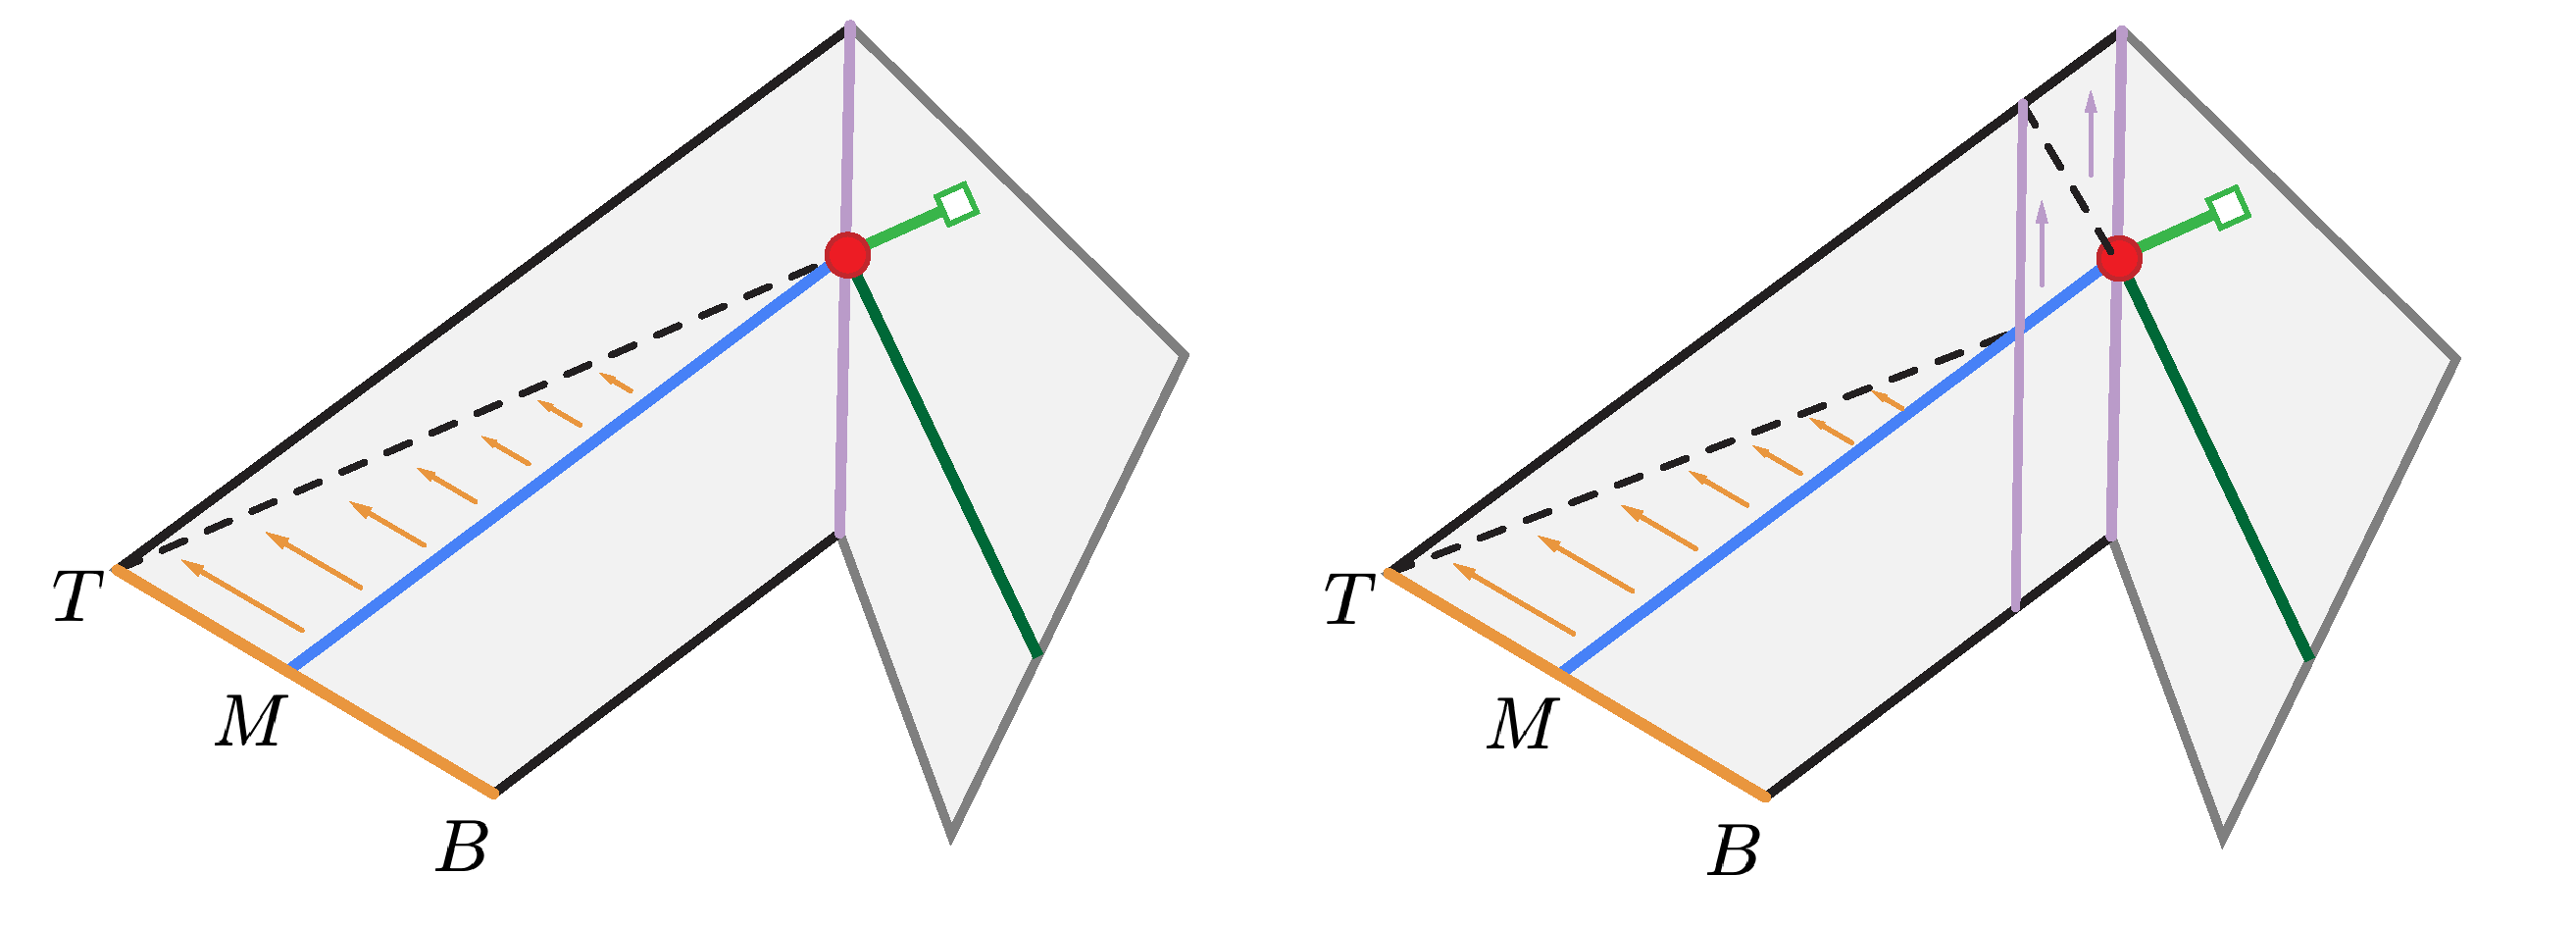
\includegraphics[width=0.9\linewidth]{prism-tex/figs/need_to_bevel}
    \caption{The vector field aligned with the pillar edge (orange) has a negative dot product with the green triangle normal; the tetrahedron with this field direction meets the green triangle at the red vertex. As a consequence, the mid-surface is not a section.
    After topological beveling, the shell becomes valid since the dot product between the green normal and the new pillar (purple) is positive.
    }
    \label{prism:fig:closed}
    
\end{figure}

Depending on the dihedral angles in the mesh $\T$,
it is possible that the dot product between one of the pillars (orange in Figure~\ref{prism:fig:closed}) and the face normals of some of the triangles from 1-ring neighborhood (green in Figure~\ref{prism:fig:closed}) is negative. 
While it may seem that this  problem could be addressed
by changing the definition so that each edge is assigned to one of the incident triangles, so that the field direction only in one incident tetrahedron needs to be considered, this problem is more significant than it may seem, as it leads to instability under small perturbations (e.g., due to floating-point rounding of coordinates). Such small perturbations can change the set of triangles intersecting a prism and thus violate the validity of the shell and, consequently, the bijectivity of $\P$.
We propose instead to refine $\T$, without changing its geometry, so that the shell corresponding to the refined mesh satisfies I2 (i.e., its middle surface is a section).
\paragraph{Topological Beveling.} We identify a prism $\Prism_v$ for which I2 does not hold and use a beveling pattern \cite{coxeter1973regular,conway2016symmetries,hart2018conway}
to decompose $\Prism_v$ in a way that $\T$ becomes a section for all 6 decompositions (I2). We refer to this operation as \emph{topological beveling}, as it does not change the geometry of the mesh, only its connectivity (Figure \ref{prism:fig:beveled_example}). 
We use the pattern in Figure \ref{prism:fig:patterns}a for $\Prism_v$, and we use the other two patterns (b) and (c) on the adjacent prisms to ensure valid mesh connectivity. The positions of the vertices are computed using barycentric coordinates (we used $t = 0.2$, i.e., the orange dot is at $1/5$ of the horizontal edge), and the normals of the newly inserted vertices are copied from the closest vertex (in Figure \ref{prism:fig:patterns}, the internal vertices have the normal of the triangle corner with the same color).

\begin{figure}
    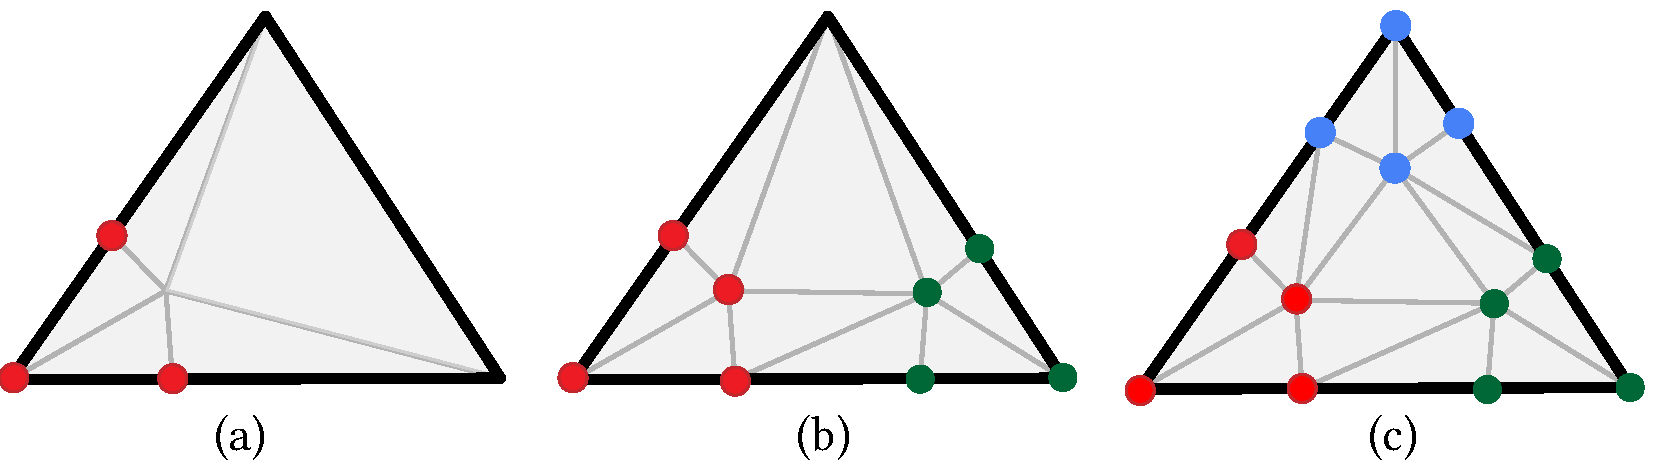
\includegraphics[width=0.9\linewidth]{prism-tex/figs/bevel}
    \caption{The beveling patterns used to decompose prisms for which $\T$ is not a section.}
    \label{prism:fig:patterns}
    
\end{figure}

\begin{figure}
    \includegraphics[width=\linewidth]{prism-tex/figs/screwdriver_bevel}
    \caption{Our algorithm refines the input model (left) with beveling patterns (middle) to ensure the generation of a valid shell. The subsequent shell optimizations gracefully remove the unnecessary vertices (right).}
    \label{prism:fig:beveled_example}
    
\end{figure}

\begin{theorem}
\label{thm:bevel}
Suppose $\T$ is the middle surface of $\S$, and neither $T_\S$ or $B_\S$ intersects with $\T$. After topological beveling, I2 holds, that is, $\T$ is a section of the shell $\S$ for all 6 decompositions.
\end{theorem}
\begin{proof}
    To show that $\T$ is a section of $\S$ we need to show that (1) $M_\Prism= \T \cap \Prism$ is a simply connected patch  for any prism of $\S$
and (2) for {each prism $\Prism$} and every point $p\in M_\Prism$ the dot product between the face normal $n(p)$ and the {pillars} $\V_i, i=1,2,3$ is strictly {positive}.

(1) is trivial since for every prism $\Prism$ of $\S$, $\Prism$ contains exactly one {triangle of the topological bevel refinement} face of $\T$.% (eventually subdivided by the beveling pattern without changing its geometry).


To prove (2), consider the dot products of the normals of each of the triangles in the beveled region sharing at least a vertex with $M_\Prism$, and the vectors along the pillars of $M_\Prism$.
We use colors to refer to the triangles of beveled prisms as shown in Figure~\ref{prism:fig:bevel-explain} left. 


\begin{figure}
    \centering
    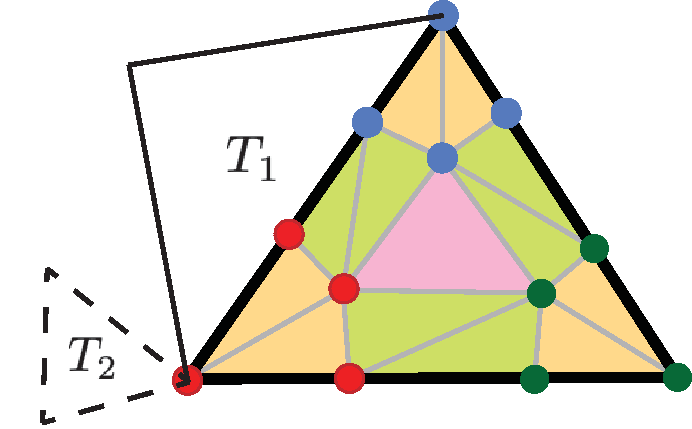
\includegraphics[width=0.5\linewidth]{prism-tex/figs/bevel_colors}
    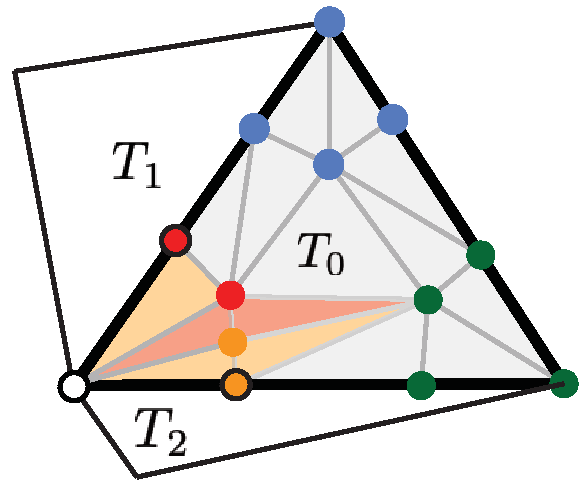
\includegraphics[width=0.4\linewidth]{prism-tex/figs/singularity-bevel-explained}
    \caption{Bevel patterns used in the proofs in Section~\ref{sec:extend-singularity}}
    
    \label{prism:fig:bevel-explain}
    \vspace{-1em}
\end{figure}
% The prism on the pink... \DZ{incomplete sentence}
The prism {corresponding to} the {pink} triangle covers only the interior of the original triangle. It satisfies {the dot product condition} since {its pillars are copied from the solution of Problem~(\ref{eq:QP})} at each vertex. 
A similar argument can be made for the green {prisms}: each  {prism} 
{gets its pillars from the edges}
incident at two of the vertices, {which are compatible with the normal of the adjacent triangle (e.g., red and blue pillars have positive dot product with  {the normal of} $T_1$).}
Finally, the prisms corresponding to orange triangles cover the same one ring that was used to compute the {original pillars (e.g., red pillar is compatible with $T_1$ and $T_2$)}. Since the same {pillar} is used for  each of the 3 vertices of the original prism, {the dot product} is {unchanged}.

\end{proof}


\paragraph{Output}
The output of this stage is a valid shell with respect to $\T$ (Section \ref{prism:sec:strong}), that is, it satisfies I1 and I2.


\subsection{Shell Optimization}
\label{prism:sec:optimization}

During shell optimization, we perform local operations
(Figure \ref{prism:fig:local_operations})
on a valid shell to reduce its complexity and increase the quality. Before applying every operation, we check the validity of the operation to ensure that: (1) the resulting middle surface will be manifold \cite{dey1999topology} and (2) the shell will be valid with respect to $\T$ (to ensure a bijective projection). We forbid any operation that does not pass these checks.  
{We would like to remark that, 
while there are different choices to guide the shell modification, we
experimentally discovered that allowing shell simplification and optimization consistently leads to thicker shells with a richer space of sections.} 

\begin{theorem}\label{thm:invariants}
Let $\S$ be a valid shell with respect to a mesh $\T$ and let $C=\{\Prism_i\}_{i\in I} \subset \S$ be a collection of prisms such that the middle surface $M_C$ of $C$ is a simply connected topological disk.

Let $\mathbb{O}$ be an operation replacing $C$ with a new collection of prisms $C'=\{\Prism_i'\}_{i\in I'}$, preserving both geometry and connectivity of the sides of the prism collection $C$, and ensuring that $M_{C'}$ is a simply connected topological disk.

If these three assumptions hold:
\begin{enumerate}
    \item property I1 holds for $C'$, %1
    \item the top and bottom surfaces of $C'$ do not intersect $\T$ ($T_{C'} \cap \T = B_{C'}\cap \T = \varnothing$), %4
    \item the dot product condition $n(p) \cdot \V(p)>0$ is satisfied for all points $p \in \T\cap \Prism_i'$ for all pillars of every prism $\Prism_i'$ of $C'$, %5
\end{enumerate}
then, $\forall i \in I'$, $\T \cap \Prism_i'$ is a simply connected topological disk.
In other words, $\T$ is a section of the new shell $\S'$ obtained by applying the operation  $\mathbb{O}$ to $\S$.
\end{theorem}
\begin{proof}

    We use $A^\circ$ to denote the interior of a set $A$. 
    We first assert that the topological disk patch $\T \cap C$ coincides with $\T \cap C'$.
    To make the notation more concise, we define $\T_C = \T \cap C$ and $\T_{C'} = \T \cap C'$.
    
    We show that $\T_C \subset C'$ by contradiction: assume there is $p\in \T_C$ but $p \not\in C'$.
    Choose a point $q \in \partial \T_C$,  that belongs to single prisms in $C$ and $C'$ and denote the enclosing prism in $C$ as $\Prism_q$ and the corresponding one in $C'$ as $\Prism_{q}'$.
    It follows from the positivity of the volumes of $\Prism_q$ and $\Prism_q'$ (Assumption 1), that there is  $\varepsilon>0$ such that the half-ball (for sufficiently small $\varepsilon$)  $\text{Ball}(q, \varepsilon) \cap \Prism_q$  coincides with $ \text{Ball}(q, \varepsilon) \cap \Prism_q'$.
    Futhermore, the validity of the initial shell guarantees that there exists an interior point $\bar{q} \in \text{Ball}(q, \varepsilon) \cap \Prism_q^\circ \cap \T$, and $\bar{q}\in \Prism_q'^\circ \cap \T \subset C'^\circ\cap \T$.
    
     Since neither $p$ or $\bar{q}$ lies on the boundary side triangles of $\partial C'$ (since $p,\bar{q}\notin\partial \T_C$), therefore there exists an interior path $P$ (i.e., a path both in $\T_C$ and in $\T_{C'}$) that connects $p$ and $\bar{q}$. By continuity the path $P$ it will cross $\partial C'$ at some point $p_i\in \T_C$. 
    Since the $\partial \T_{C'} = \partial \T_C$ is a fixed boundary loop (by the definition of $\mathbb{O}$), and does not contain interior points, $p_i$ can only cross on the top surface or bottom surface of $C'$ which contradicts Assumption 2. The roles of $C$ and $C'$ can be inverted to complete the proof. 
    
    We then  map $M_C$ to a
    regular planar $n$-gon $D$, with vertices on $\partial M_C$ mapped cyclically to the vertices of $\partial D$.
    It follows from \cite[Corollary 6.2]{floater2003one} that such a convex combination mapping $\varphi\colon M_C \to D$ is bijective. Then, similarly to the construction in Theorem~\ref{thm:projection},
    we 
    %``lift'' $D$ and 
    define $\phi\colon C \to D\times[-1,1]$ through affine mapping induced by the thetrahedralization of the prisms $\Prism_i$.
    %
    Similarly, we define $\psi \colon C' \to D\times[-1,1]$. The mapping $\psi$ is also bijective because of Assumption 1 and the definition of $\mathbb{O}$ it follows that the codomain of $\psi$ is the same as $\phi$.
    %
    Note that in both cases, the map transforms the vector field $\V(p)$ to the constant vector field $e_z = (0,0,2)$, and the projection is $\P_z$, as defined in the proof of Theorem~\ref{thm:projection}. 
    
    The dot product condition (Assumption 3) ensures that $\P_z$ defines a bijection between $D$ and $\psi(\T_C)${;} and further, the image {satisfies} $\P_z(\psi(\Prism_i'\cap \T)) = \psi(M_i')$ where $M_i'$ is the middle surface (a single triangle) of $\Prism_i'$.
    Therefore, since $\psi$ and $\P_z$ are both continuous and bijective, they are homeomorphisms which preserve topology, 
    thus $\Prism_i'\cap \T $ is a simply connected topological disk.
\end{proof}


We note that assumption (2) in Theorem~\ref{thm:invariants} prevents the input surface from crossing the bottom/top surface, thus avoiding it to move in the interior of a region covered by more than one prism. 

Our local operations (satisfying the definition of $\mathbb{O}$ in Theorem \ref{thm:invariants}) are translated from surface remeshing methods \cite{dunyach2013adaptive} since our shell can be regarded as a triangle mesh (middle surface) extruded through a displacement field $\N$. All the local operations described below directly change the middle surface, and consequently affect the extruded shell. After every operation, the middle surface is recomputed by intersecting $\T$ with the edges of the prisms in $\S$.
%\DZ{This is not clear,expand}
\begin{figure}
    \centering
    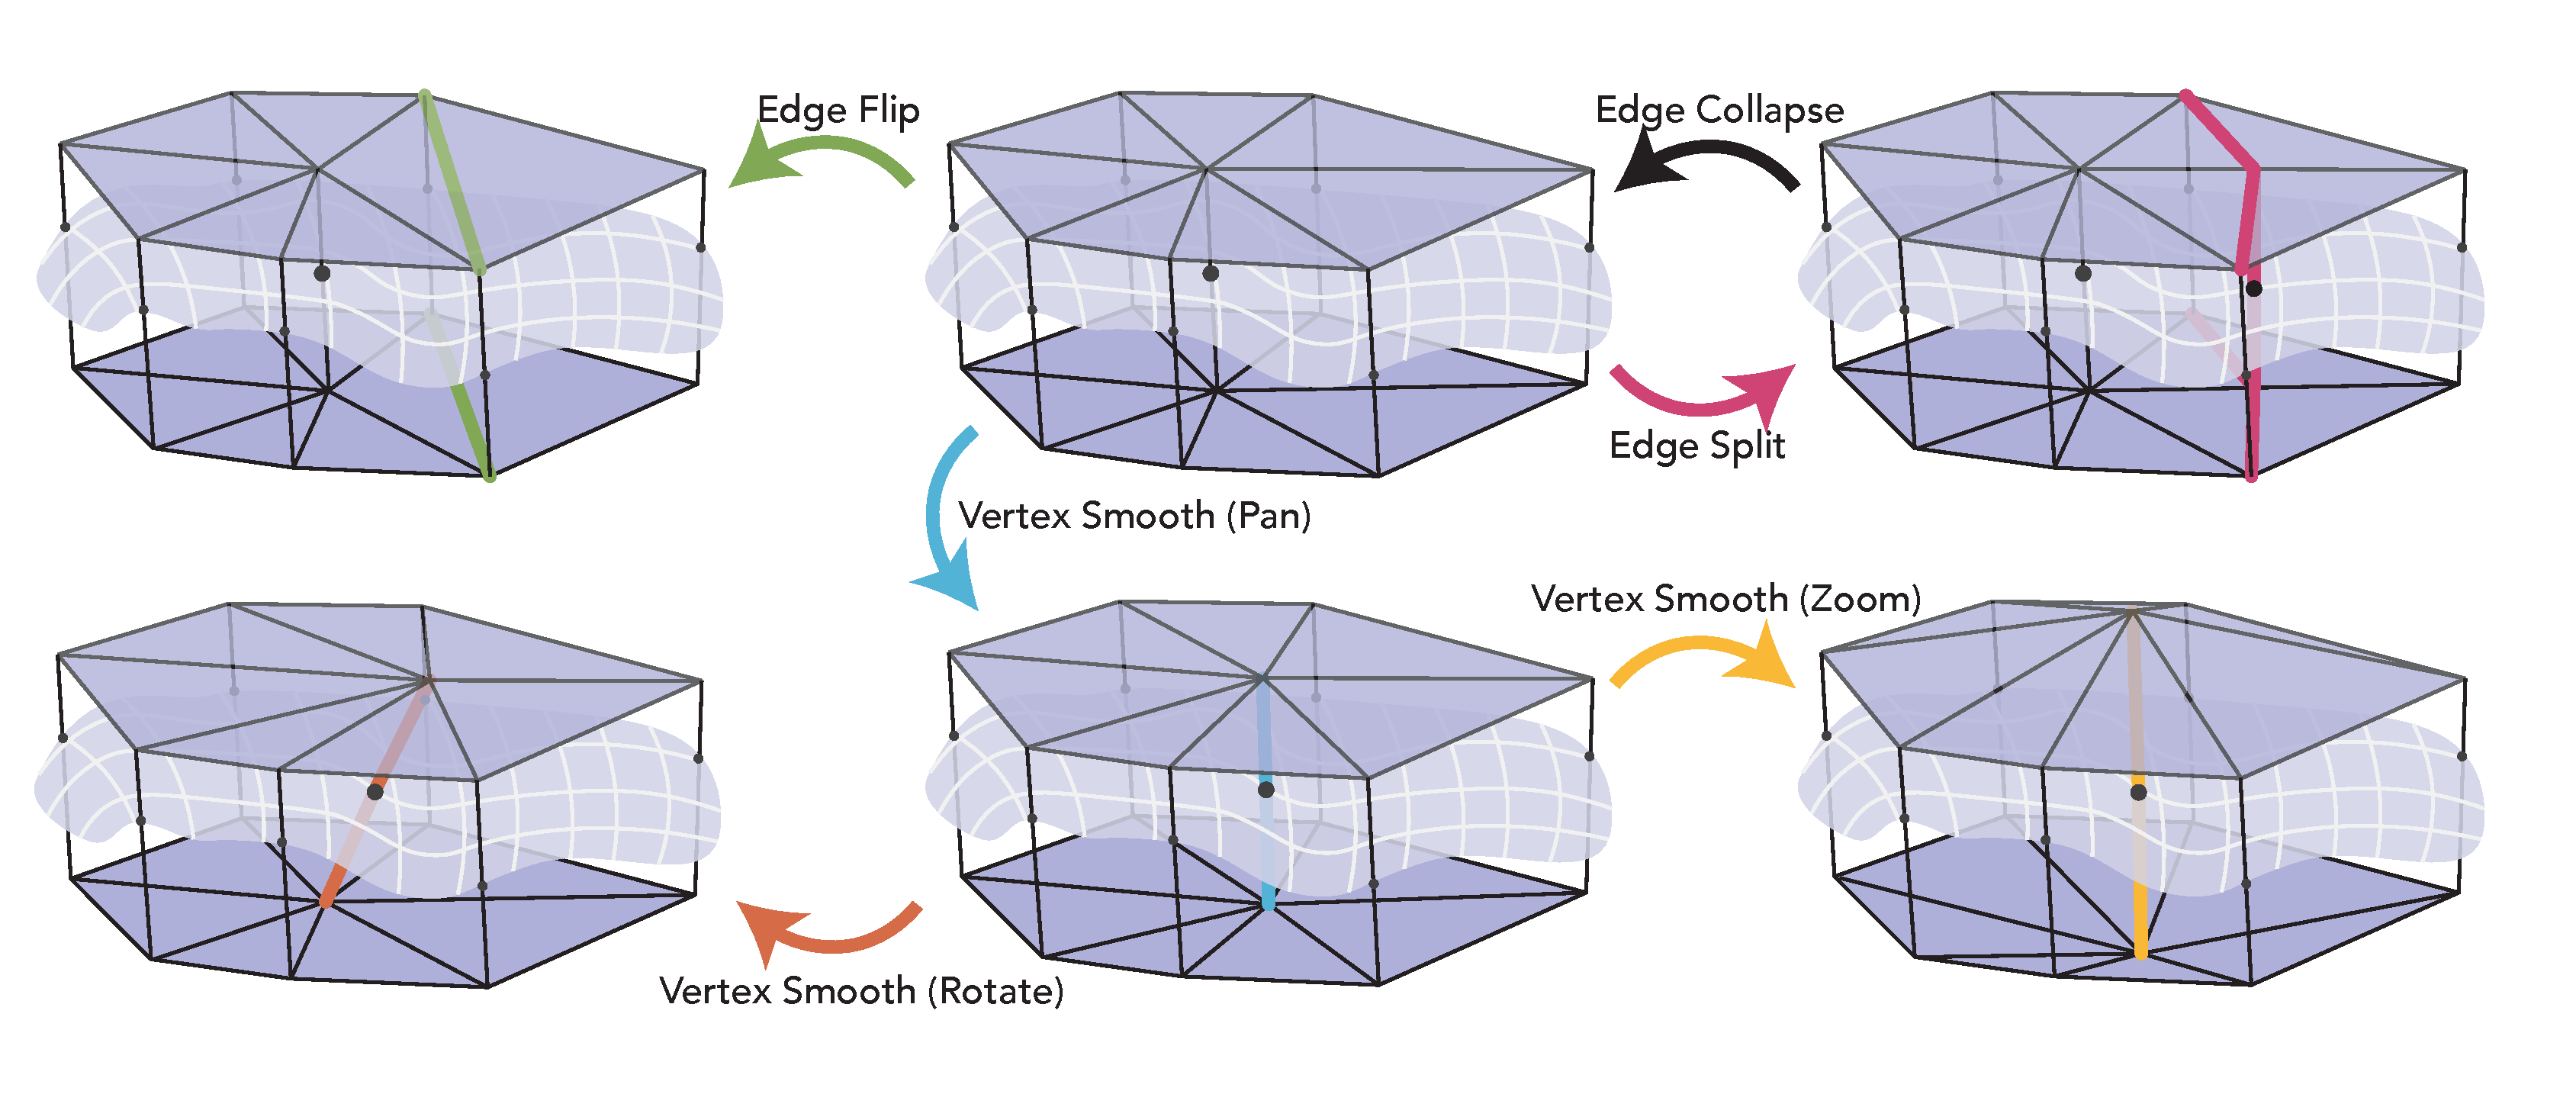
\includegraphics[width=0.9\linewidth]{prism-tex/figs/local-operations}
    % \includegraphics[0.5\linewidth]{prism-tex/figs/block_singular}
    \caption{Different local operations used to optimize the shell. Mesh editing operations translate naturally to the shell setting. For vertex smoothing, we decompose the operation into 3 intermediate steps: pan, zoom, and rotate.}
    \label{prism:fig:local_operations}
    
\end{figure}

\paragraph{Shell Quality}
We measure the quality of the shell $\S$ using the MIPS energy \cite{hormann2000mips} of its middle surface $M_\S$. For each triangle $T$ of the middle surface, we build a local reference frame, and  compute the affine map $\J_T$ transforming the triangle into an equilateral reference triangle in the same reference frame. The energy is then measured by
\begin{equation*}
    \sum_{T \in M_\S} \frac{\tr(\J_T^T\J_T)}{\det(\J_T)}.
\end{equation*}
This energy is invariant to scaling, thus allowing the local operations to coarsen the shell whenever possible while  encouraging the optimization to create well-shaped triangles. Good quality of the middle surface decreases the chances, for the subsequent operations, to violate the shell invariants.

\paragraph{Shell Connectivity Modifications.} We translate three operations for triangular meshes to the shell settings (Figure~\ref{prism:fig:local_operations} top). Edge collapse, split, and flip operations can be performed by simultaneously modifying the top and bottom surfaces
and retrieve the positions for the middle surface through the intersection. We only accept the operations if they pass the invariant check.

\paragraph{Vertex Smoothing.} Due to the additional degree of freedom on vertex-pairs (position, direction, and thickness), we decompose the smoothing operations into three {components} (Figure~\ref{prism:fig:local_operations} bottom). 
\emph{Pan} moves the positions of the top and bottom vertex at the same time, 
minimizing the MIPS quality of the middle surface. Neither the thickness or direction will be changed. 
\emph{Rotate} re-aligns the local direction to be the average of the neighboring ones while keeping the position of the middle vertex fixed. 
\emph{Zoom} keeps the direction and position of the middle vertex, and set the thickness of both top and bottom to be 1.5 times of the neighbor average, capped by the input target thickness.


\paragraph{Invariant Check}
% Our algorithm maintains both invariants using exact predicates \cite{shewchuk1997adaptive}. 
We use exact orientation predicates \cite{shewchuk1997adaptive} to make sure all the prisms satisfy positivity (I1). Further, we ensure that the original surface $\T$ is not intersecting with the bottom and top surface, except at the prescribed singularities.
The check is done using the triangle-triangle overlap test \cite{guigue2003fast}, accelerated using a static axis-aligned bounding box tree constructed from $\T$. 
To accelerate the checks for normal condition, 
for each prism $\Prism_i$, 
we maintain a list triangles overlapping with its convex hull (an octahedron), 
and check their respective normals against all the three pillars of $\Prism_i$. These three checks ensure that the three conditions in  Theorem~\ref{thm:invariants} are satisfied.
%
Note that the vertex smoothing operation is continuous, in the sense that any point between the current position and the optimal one improves the shell. 
We, however, handle it as a discrete operation to check our conditions: we attempt a full step, and if I1 is not satisfied, we perform a bisection search for a displacement that does. We avoid bisection for the other two conditions since they are expensive to evaluate.



\paragraph{Projection Distortion} 
An optional invariant to maintain (not {necessary} for guaranteeing bijectivity, but useful for applications), 
is a bound  on the maximal distortion $\D_\P(\Prism) $ of $\P$ for a prism $\Prism$. 
We measure it as  the maximal angle between the normals of the set $\C$ containing the faces of $\T$ intersecting $\Prism$ and $\V$:
\begin{equation*}
    \D_\P(\Prism) = \max_{p \in \C} \angle (n_p, \V(p)),
\end{equation*}
where $\angle$ is the unsigned angle in degrees. This quantity is bounded from below by the smallest dihedral angle of $\T$, making it impossible to control exactly. However, we can prevent it from increasing by measuring it and discarding the operations that increase it. In our experiments, we use a threshold of $89.95$ degrees.

\paragraph{Scheduling and Termination}
Our optimization algorithm is composed of two nested loops. The outer loop repeats a set of local operations until the face count between two successive iteration decreases by less than 0.01\%. In the inner loop we: (1) flip every edge of $\S$ decreasing  the MIPS energy and avoiding high and low vertex valences \cite{dunyach2013adaptive}; (2) smooth all vertices which include pan, zoom, and rotate; and (3) collapse every edge of $\S$ not increasing the MIPS energy over {30}. Note that for every operation, we check the invariants, the projection distortion, and manifold preservation and reject any operation violating them.
%
After the outer iteration terminates (i.e.  the shell cannot be coarsened anymore), we further optimize the shell with 20 additional iterations of flips and vertex smoothing.




% \TS{new text done with Zhongshi, old text is on the bottom, probably kill it}

% We separate the operations into \emph{outer passes, which contains only one of the operations (either collapse, flip or smooth), and}
% iteratively perform \emph{outer passes} composed of one sequence of edge collapse, one of edge flip, and one of vertex smoothing. We stop these iterations when the face count between different passes decreases by less than 0.01\%. We then further optimize the shell with 20 additional passes of flips and vertex smoothing.

\begin{figure}
    \centering
    \includegraphics[width=\linewidth,draft=false]{prism-tex/figs/doublewheel_pinch}
    % \includegraphics[0.5\linewidth]{prism-tex/figs/block_singular}
    \caption{A model with 48 singularities and a close up around one (left).
    Our shell is pinched around each of them without affecting other regions (right).}
    \label{prism:fig:singularity_example}
    
\end{figure}


\subsection{Singularities}\label{prism:sec:singularities}

% We introduced the algorithm assuming that problem \eqref{eq:OPT} always has a solution, and assuming that our mesh does not contains boundaries. We will now extend our construction to handle these cases, which requires minor variations to our algorithm.

Singularities, i.e. vertices of $\T$ for which the constraints set of problem \eqref{eq:OPT} is empty, are surprisingly common in large datasets (Figure~\ref{prism:fig:singularity_example} shows an example). For instance, in our subset of Thingi10k \cite{zhou2016thingi10k}, although only 0.01\% vertices are singular,  8\% of the models have at least one singular point. This has been recently observed as a limitation for the construction of nested cages \cite[Appendix A]{sacht2015nested}, and it is a well-known issue when building boundary layers \cite{aubry2015most,aubry2017boundary,garimella2000boundary}.
%
There are two main situations that give rise to singular points. 
The first one naturally generates a singular point when more than two ridge-lines meet (e.g., figures~\ref{prism:fig:singularity_example} and~\ref{prism:fig:singularity-boolean}), thus making the point a feature point. 
The second one is a pocket-like mesh artifact, often produced as a result of mesh simplification (Figure~\ref{prism:fig:singularity-illustration}).

While singularities might seem fixable by applying local smoothing or subdivision as a pre-process, it is not desirable in the case of a feature point, and is likely to introduce self-intersection or more serious geometric inconsistency.
%in the presence of the meshing artifacts.
Therefore, due to the above reasons and observing that they are very uncommon, we propose to extend our theory (Section~\ref{sec:extend-singularity}) and algorithm to handle isolated singularities  by \emph{pinching} the thickness of the shell. Note that in the rare case where two singular points are sharing the same edge, they are \emph{automatically} separated by our topological beveling.

\paragraph{Pinching.} 
We extend our definition of the shell by allowing it to have zero thickness on singularities, thus tessellating the degenerate prism with 4 instead of 6 tetrahedra (Figure~\ref{prism:fig:singularity-illustration}). We further remark that these isolated points must be excluded from Definition~\ref{def:section}. In the implementation, this requires to change the intersection predicates to skip the singular vertices.
With this change, the singularity becomes a trivial point of the projection operator $\P$,
% \DZ{all middle surface points are fixed points of $\P$}
and the rest of our shell can still be used in applications without further changes. Since singularities tends to be isolated (they are usually located at the juncture of multiple sharp features), this solution has minimal effects on applications: for example, when our shell is used for remeshing, pinching the shell at singularities will freeze the corresponding isolated vertices while allowing the rest of the mesh to be freely optimized.

\begin{wrapfigure}{r}{0.3\linewidth}
    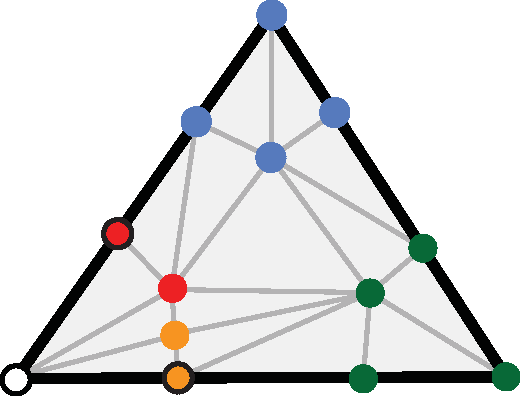
\includegraphics[width=1\linewidth]{prism-tex/figs/singular_bevel}
\end{wrapfigure}

\begin{figure}
\centering
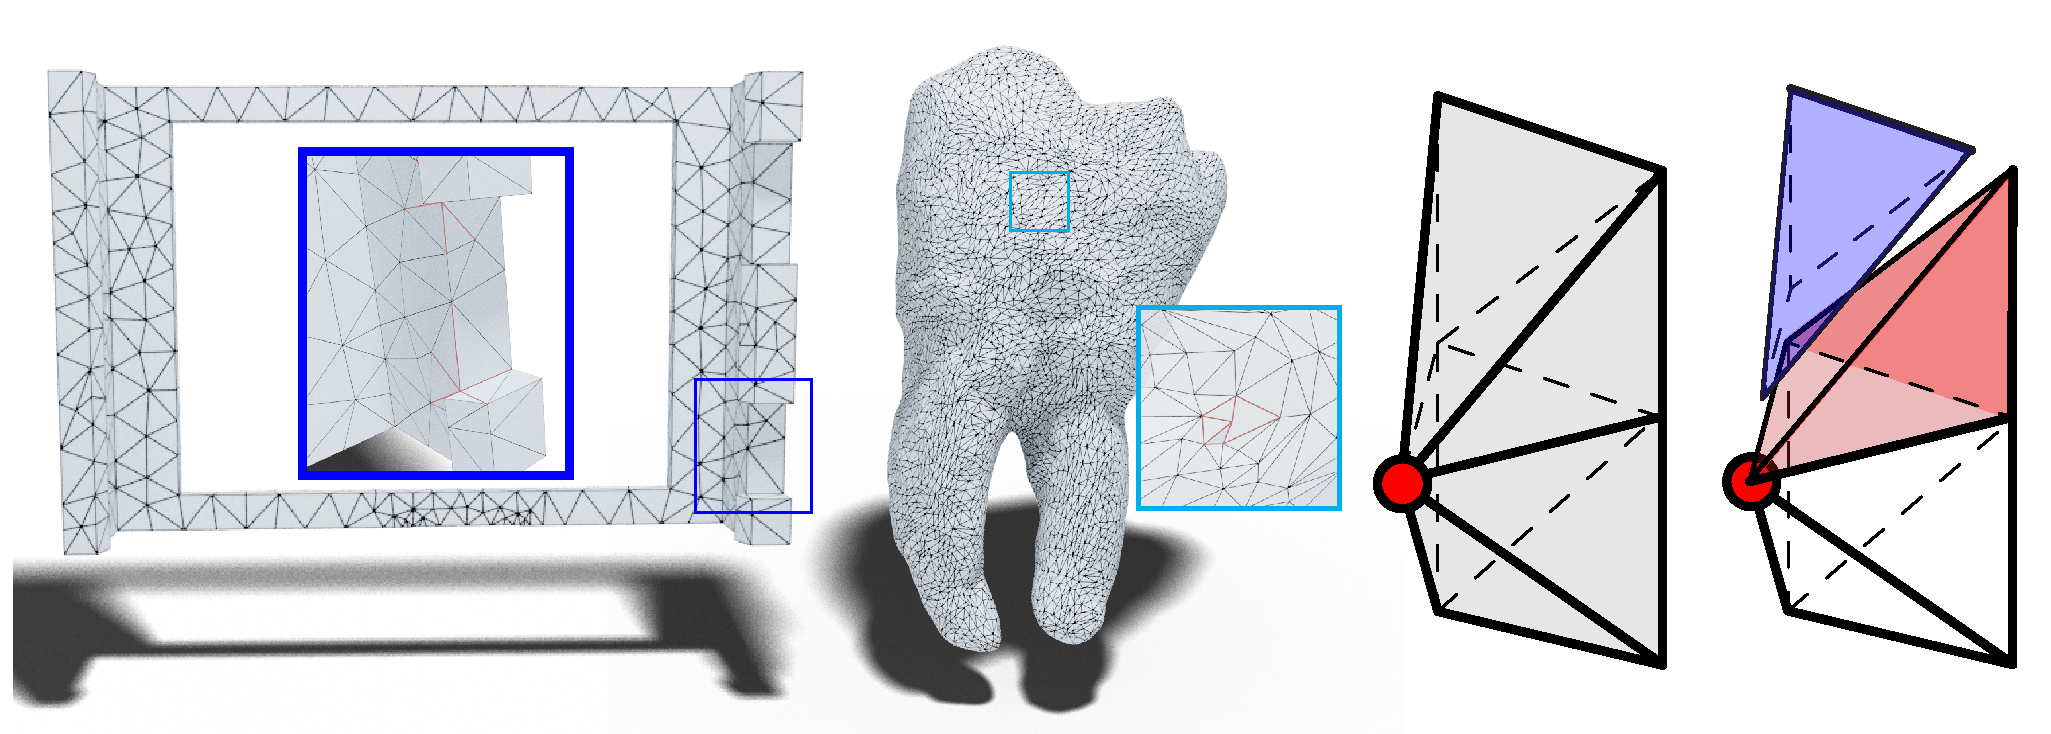
\includegraphics[width=\linewidth]{prism-tex/figs/degenerate_prism_decompose}
\caption{Left to right: examples of a singularity as a feature point and as a meshing artefact; and illustration of the degenerate prism with a singularity (red) and its tetrahedral decomposition made of only four tetrahedra.}
\label{prism:fig:singularity-illustration}

\end{figure}

The topological beveling algorithm is changed most significantly: for singularities, there is no pillar to copy from.
In this case, we apply an additional edge split, to use the pattern in the inset (with the singularity marked by a white dot) in the one-ring neighborhood of the singularity.
The newly inserted vertices lie either inside a triangle (uncircled red and orange dots), 
or in the interior of an edge (circled red and orange dots).
Therefore, we assign to the orange vertices the average normal of the two adjacent triangles, and to red the pillar of the connected orange one.


Additionally, the edges connecting singularities will always be beveled/split after beveling. Therefore no prism will contain more than one singular point.
We discuss the technical extensions for our proofs to shells with pinched prisms as follows,

\subsection{Extension to meshes with Singularities}\label{sec:extend-singularity}
Most of the proofs and definition in Section~\ref{prism:sec:method} easily extends to meshes with singularity or pinched shells. For instance,
{both} Theorem~\ref{thm:projection} and Definition~\ref{def:validshell} apply to pinched shells by just considering a prism made of 4 (2 for the top and 2 for the bottom slab) instead of 6. Propositions~\ref{thm:I1} and~\ref{thm:thickness} both rely on per-vertex properties; by just excluding singular vertices (and neighboring prism) from the statements the proofs (and our algorithm) still holds.


Theorem~\ref{thm:invariants} requires some minor additional considerations. As a consequence of beveling, no two singularities are adjacent. Therefore, we can always find a point $q \in \partial \T_C$ that belongs to a single prism (Appendix~\ref{app:invariant-checks}) since every prism will have a positive volume
because no singularities are adjacent.


Finally Proposition~\ref{thm:bevel} requires a new proof since the beveling pattern used for singularities is different.
% \begin{proposition}
% For a prism $\Prism$ with one singularity, 
% \end{proposition}
\begin{proof}
In  Figure~\ref{prism:fig:bevel-explain} right, we highlight in red and orange the triangles not covered by the discussion in Appendix~\ref{app:bevel}. 
The prism corresponding to an orange middle triangle intersects the edge-adjacent triangle. And since the new pillars are computed as the average of the normals of the two adjacent triangles with dihedral angle strictly less than $360^\circ$ 
 (Section~\ref{prism:sec:singularities} inset), each dot product is positive. 
The prism {for} a pink middle triangle intersects only the interior of the original triangle, and the dot product between the pillars and the triangle normal are positive by construction. 
\end{proof}



\begin{figure}
    \centering
    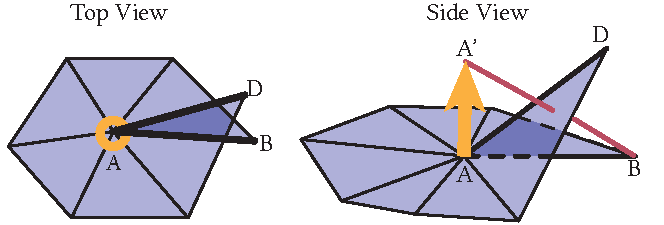
\includegraphics[width=0.9\linewidth]{prism-tex/figs/boundary_singular}
    \caption{$AA'$ is a direction with positive dot product with respect to all its neighboring faces. However, no valid shell can be built following that direction.}
    \label{prism:fig:boundary_singularity}
    
\end{figure}

\subsection{Boundaries.}\label{prism:sec:boundaries}

We introduced our algorithm, assuming that the input mesh does not have boundaries. We will now extend our construction to handle this case, which requires minor variations to our algorithm.

For some vertices on the boundary, it might be impossible to extrude a valid shell (Figure~\ref{prism:fig:boundary_singularity}), even if problem \eqref{eq:OPT} has a solution, as  Theorem~\ref{thm:thickness} does not apply in its original form. 
%
We identify such cases by connecting every edge in the 1-ring neighborhood of the boundary vertex
to the extruded point and check if they collide with the existing 1-ring triangles (e.g., the triangle $A'AB$ intersects the existing input triangle in Figure~\ref{prism:fig:boundary_singularity}). If it is the case, we consider this vertex as a singularity, and we pinch the shell. Note that this is an extremely rare case and, in our experiments, we detected it only for models where the loss of precision in the STL export introduces rounding noise on the boundary.% (and the problem goes away increasing precision). We could not identify any realistic case of this scenario in our model collection.

Once we pinch all boundary singularities, our construction extends naturally to the boundary. The only necessary modification is in the shell optimization (Section~\ref{prism:sec:optimization}), where we skip all operations acting on boundary vertices to maintain the bijectivity of the induced projection operator (Figure~\ref{prism:fig:open-hand}).
%
We thus freeze these vertices and never allow them to move or be affected by any other modification of the shell. Note that, in certain applications, it might also be useful to freeze additional non-boundary vertices to ensure that these remain on the middle surface during optimization (e.g., to exactly represent a corner of a CAD model).


\begin{figure}
    \centering
    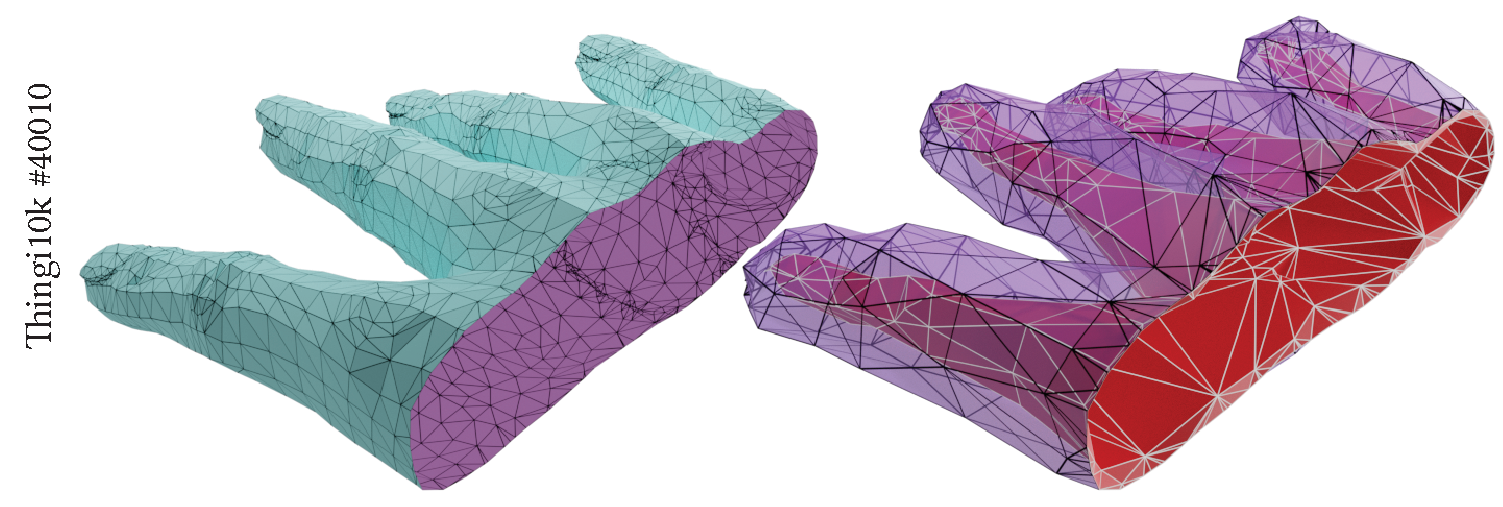
\includegraphics[width=0.9\linewidth]{prism-tex/figs/open-hand}
    \caption{An example of a mesh with boundary.}
    \label{prism:fig:open-hand}
    
\end{figure}




.